\chapter{Introduction}\label{ch:introduction}

Machine learning is highly difficult. It’s what mathematicians call an “NP-hard” problem. That’s because building a good model is really a creative act. As an analogy, consider what it takes to architect a house. You’re balancing lots of constraints -- budget, usage requirements, space limitations, etc. -- but still trying to create the most beautiful house you can. A creative architect will find a great solution. Mathematically speaking the architect is solving an optimization problem and creativity can be thought of as the ability to come up with a good solution given an objective and constraints. Classical computers aren’t well suited to these types of creative problems.Machine learning algorithms are tasked with extracting meaningful information and making predictions about data. In contrast to other techniques, these algorithms construct and/or update their predictive model based on input data. The applications of the field are broad, ranging from Spam filtering to image recognition, demonstrating a large market and wide societal impact.\par\bigskip
In recent years, there have been a number of advances in the field of quantum information showing that particular quantum algorithms can offer a speedup over their classical counterparts. Execution time is just one concern of learning algorithms. Quantum optimizations are capable of finding the global minimum of a non convex objective functions in a discrete search space. Storage capacity is also of interest. Quantum associative memories store exponentially more patterns than a classical Hopfield networks. In addition to supplying exponential speed-ups in both number of vectors and their dimension, quantum machine learning allows enhanced privacy: In a Quantum clustering algorithm only $O(log(MN))$ calls to the quantum data-base are required to perform cluster assignment, while $O(MN)$ are required to uncover the actual data \cite{kmeans}.\par\bigskip
\section{Deep Learning: The boom}
\begin{figure}[H]
\centering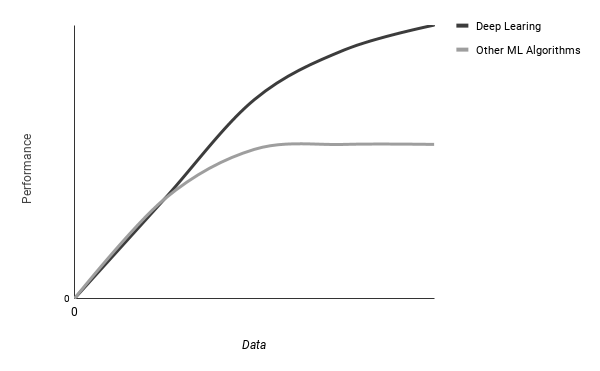
\includegraphics[width=.6\textwidth]{images/chart.png}
\caption{Deep learning vs Traditional Machine Learning}
\end{figure}
Now the main question, why this field is getting boomed now a days ? The first Convolutional Neural Network was developed by Yann LeCun in 1995 \cite{lecun} why did it take so long for deep learning to take off? One Answer, The Scale. Scale drives deep learning progress, Scale in both data-set sizes and computational power. But the same scale could act as bottleneck for deep learning.\par\bigskip
The data volumes are exploding, more data has been created in the past two years than in the entire previous history of the human race. Data is growing faster than ever before and by the year 2020, about 1.7 megabytes of new information will be created every second for every human being on the planet. By then, our accumulated digital universe of data will grow from 4.4 zettabyets today to around 44 zettabytes, or 44 trillion gigabytes. The demand for storage has grown more than 50\% annually in recent years, a rate faster than the rapidly decreasing unit cost of storage. The growth of data is profound and there are no signs of it slowing. Moore’s law has taught us that we will see a doubling every 18 months. That means a 1TB footprint today will increase to 16TBs in 6 years. There is an inconvenient truth in technology: The amount of data keeps growing exponentially, while the increases in the power of computers are slowing down. Computers today can carry out those instructions in nanoseconds, but they still do it one step at a time, which has become a liability known as the von Neumann bottleneck. If individual chips can no longer be made faster, and the amount of work computers have to do continues to grow, the only way to attack ever larger data problems with von Neumann programmable computers will be to build more computers and ever bigger data centers. It seems as though we have hit a wall in growth of computational capacities. How can we meet this demand for data storage and computational power? One of most promising solution is Quantum computers and Quantum information processing.
\section{How can Quantum Computers Help?}
The basic idea is to use the atypical behavior of quantum physics such as quantum tunneling and quantum entanglement to get atoms to make calculations. A dozen atoms in a quantum computer would be more powerful than the world’s biggest supercomputer. While regular computers symbolize data in bits, 1s and 0s expressed by flicking tiny switch-like transistors on or off, quantum computers use quantum bits, or qubits, that can essentially be both on and off, enabling them to carry out two or more calculations simultaneously. In principle, quantum computers could prove extraordinarily much faster than normal computers for certain problems because they can run through every possible combination at once. In fact, a quantum computer with 300 qubits could run more calculations in an instant than there are atoms in the universe. Also Qubits can store more data than classical bits, n qubits can carry about $2^n$ classical bits of information due to superposition.
